\documentclass{article}
\usepackage{graphicx}


\begin{document}


% Title Page
\title{Data Collection Documentation (Draft)}
\author{Steven Deutekom}
\date{June 2019}
\maketitle


% Table of Contents
\newpage
\tableofcontents


% Introduction %%%%%%%%%%%%%%%%%%%%%%%%%%%%%%%%%%%%%%%%%%%%%%%%%%%%%%%%%
\newpage
\section{Introduction}
% What are we doing?
The goal of this project is to collect source code samples from individual authors from various online sources. It requires finding samples that have certain sociolinguistic characteristics such as gender, region, and experience. In addition to sociolinguistic characteristics, it is necessary that the samples are the work of only a single author. Data that meets these needs is being collected and used to create a dataset with information on authors and their source code.

% Why are we doing it?
The collected data will be used for sociolinguistic research into how people use programming languages. Current and future University of Lethbridge students will use this research to learn how sociolinguistic characteristics affect how programmers write code. Previous research was conducted with a small dataset of student programs. This new dataset will contain many samples from a larger set of programmers.

% What is coming in this documents?
The document is broken into three main sections. Each section details one of the sources that was used to collect data. First, the collection methods used to gather source code from GitHub. Then, the methods used to collect source code from Codeforces. Lastly, the methods that were used to add gender data to the samples collected.

Each section introduces the sources and collection methods. Then it discusses the pros and cons of the source. Next an overview of the process of collecting data is given, with diagrams to help visualize it. Following this a more in depth technical examination of the collection process takes place. Finally, some reflection on the source is given (needed?).


% Github %%%%%%%%%%%%%%%%%%%%%%%%%%%%%%%%%%%%%%%%%%%%%%%%%%%%%%%%%%%%%%%
\section{Collecting Source Code From GitHub}


%& Introduction to the sources being used
\subsection{Data Sources}


%% Introduction to the collection strategies
\subsection{Collection Startegies}


%% Pros and Cons of each along with steps taken to try and overcome any issues.
\subsection{Pros And Cons}


%% High level overview of the process w/ diagrams
\subsection{Process Overview}

%%% Ght and Big Query process
\subsubsection{GhTorrent and Google Big Query}

% Process Diagram
\begin{figure}[!h]
    \centering
    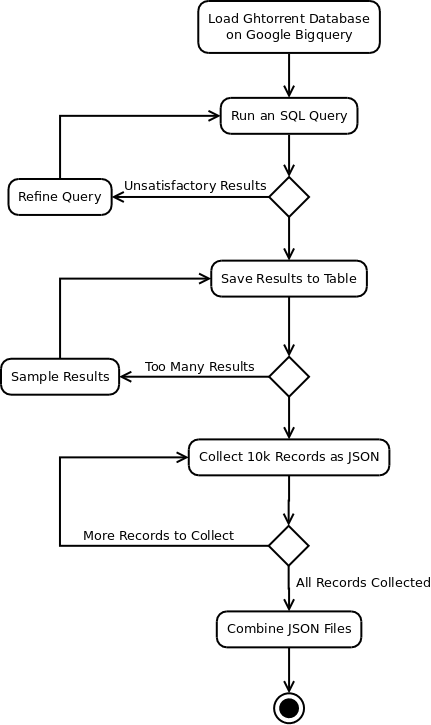
\includegraphics[height=10cm]{diagrams/ght_process.png}
    \caption{Getting Data From Ghtorrent}
\end{figure}

%%% Git projects process
\subsubsection{Collecting Git Projects}

% Process Diagram
\begin{figure}[!h]
    \centering
    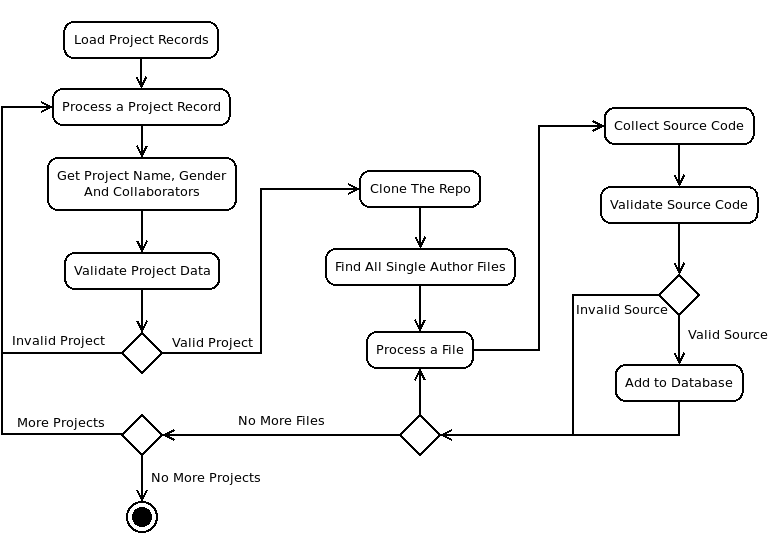
\includegraphics[height=8cm]{diagrams/projects.png}
    \caption{Getting GitHub Project Source Code}
\end{figure}

%%% Git commits process
\subsubsection{Collecting Git Commits}

% Process Diagram
\begin{figure}[!h]
    \centering
    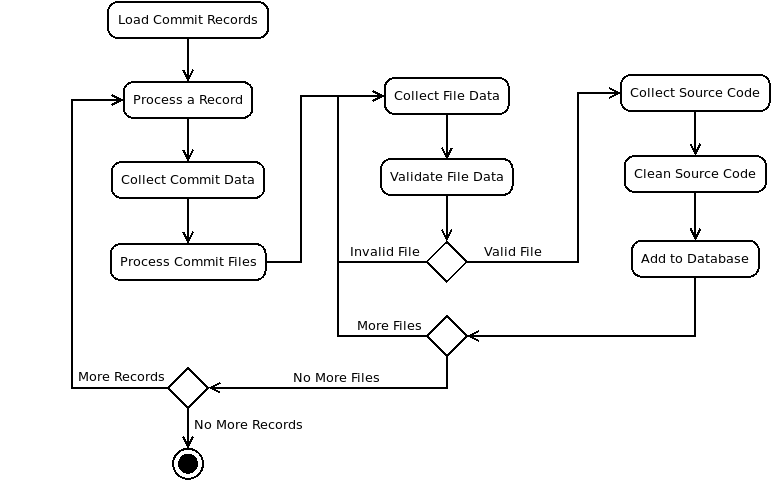
\includegraphics[height=7.5cm]{diagrams/commits.png}
    \caption{Getting GitHub Commit Source Code}
\end{figure}


%% Discussion of each subprocess with technical details and the data it gives and technical issues that are not related to the websites themselves (not listed in pros and cons)
\subsection{Process Details}

%%% Ght and Big Query process
\subsubsection{GhTorrent and Google Big Query}

\paragraph{Process}
\paragraph{Data}
\paragraph{Additional Issues}

%%% Git projects process
\subsubsection{Collecting Git Projects}

\paragraph{Process}
\paragraph{Data}
\paragraph{Additional Issues}

%%% Git commits process
\subsubsection{Collecting Git Commits}

\paragraph{Process}
\paragraph{Data}
\paragraph{Additional Issues}

% Codeforces %%%%%%%%%%%%%%%%%%%%%%%%%%%%%%%%%%%%%%%%%%%%%%%%%%%%%%%%%%%
\section{Collecting Source Code From Codeforces}


%% Introduction to the source being used %%
\subsection{Sources}


%% Pros and cons of collecting from codeforces along with steps taken to try and overcome any issues. %%
\subsection{Pros And Cons}


%% High level overview of the process %%
\subsection{Process Overview}

\begin{figure}[!h]
    \centering
    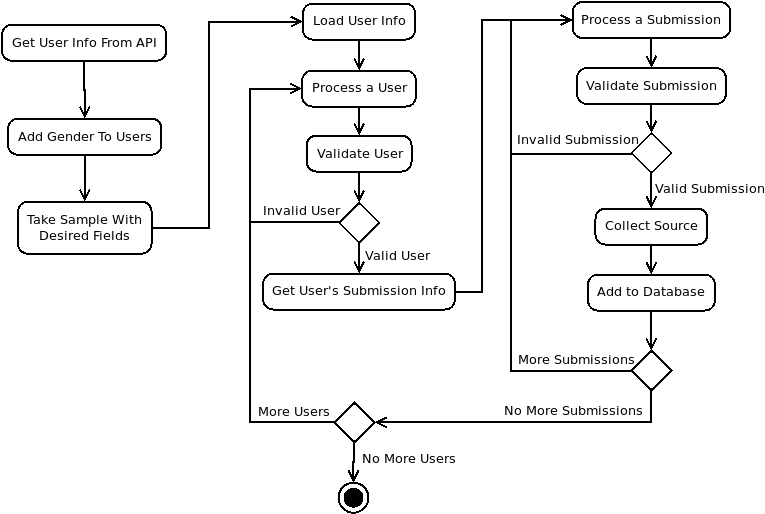
\includegraphics[height=8cm]{diagrams/cf_process.png}
    \caption{Getting Data From Codeforces}
\end{figure}


%% Discussion of each subprocess with technical details, the data collected, and the technical issues %%
\subsection{Process Details}

%%% Using selenium webdriver
\subsubsection{Using Selenium}

\paragraph{Process}
\paragraph{Data}
\paragraph{Additional Issues}

%%% Using the direct links only
\subsubsection{Using Links Only}

\paragraph{Process}
\paragraph{Data}
\paragraph{Additional Issues}


% Gender Labeling %%%%%%%%%%%%%%%%%%%%%%%%%%%%%%%%%%%%%%%%%%%%%%%%%%%%%%
\section{Adding Gender Labels}
One of the sociolinguistic features that is important to the project is Gender. Unfortunately, gender is available for authors on Github or Codeforces. Since it cannot be collected along with author information gender must be obtained in other ways. This can be done using an authors first name. There are a number of websites and APIs available that offer gender data for first names. All the gender information for authors in the dataset were gathered in this way.

%% Introduction to the sources being used %%
\subsection{Sources}
There are several websites and APIs for adding gender for first names. They include gender-api.com, genderize.io, namsor.com, and nameapi.org. This project primarily used genderize.io because it is free and allows 1000 name lookups per day. In addition to this a table was kept in the database to store the names that were already known. The service offers a 'male', 'female', or 'unknown' verdict when given a name. It also gives a probability that a result is correct (from sample?). In addition it is possible to pass a country code to along with the name to obtain results that are more specific? The other APIs all offer similar services, but they all require monthly payment for more than a small number of name guesses.

%% Discussion of the pros and cons and difficulties along with steps taken to try and overcome any issues. %%
\subsection{Pros And Cons}
Inferring gender from names is not an easy task (some examples and sources). It is also not always very clear how a service is determining the gender (cite). So this is immediately a problem. The probability given can help to determine the likelihood of results being correct, but it still is only as good as the service. There are some stats given by (info and paper citation) that comment on the accuracy of the above 4 services.

Aside from the accuracy of these methods being suspect, the major con is that for the most part they are paid services. Some of them do offer free limits, but only genderize is really worth it for any larger needs, and even then only with an offline backup of already labeled names. The good news is that there are many people sharing a small number of names, so a large number of samples can be labeled with a small database.

People are not always truthful with their names on these profiles, sometimes they do not even give a name. As a result there are fewer samples to work with if gender is desired. If country is going to be used to add accuracy to the label then it lowers the number of samples available further.

It is possible though with several sources available that when a selection of samples is made they can have their gender labels confirmed by other sources. Because many people share a similar name it is also not as big a deal to use free credits or even pay for a small period to obtain better results for a set of good samples.

All services are less effective at labeling Asian names (citation). This can present a problem for datasets that are using large numbers of samples from Asian countries.

This is really the only way other than contacting authors directly to find out their gender. Which would be problematic with any reasonably sized database. Not to mention many people would be unlikely to respond to such a question.

It is also worth noting that these methods also are firmly gender binary. They do not take into account any other factors. And the connection between gender of a name and biological sex is by no means guaranteed.

It is not always clear wether a country should be used, though it is suggested that this improves the results (cite).

The number of samples can be low for a name so even if the probability is high it is not really certain if the sample size is large enough.

The names collected show a much less accurate probability for female names. Most male names are classed as 0.9-1.0 and more female names fall into this category, but in some cases at most half of the names are in the 0.9-1.0 category. This suggests that there are some issues with classifying female names properly. Wether it is that more female names are unisex or that there are low samples for them is unknown (to me. Could put in a table).


%% Overview of the process %%
\subsection{Process Details}
\subsubsection{Process}
The process used for collecting gender for names is relatively simple. Given a name the database is checked to see if it has the name already. If the name is not in the database it is looked up with the genderize.io API. If the API returns a result that result is added with the name to the database. If the API limit has been reached then a appropriate(what?) response is given. The scripts all have options (Do they?) to save results for later processing if gender cannot be determined. If there name is able to be labeled then the label and the probability are returned.

The labels added to the scripts do not use country codes. As stated above it will be desireable to re-label the names on samples that are used by submitting the names and countries again to other APIs to see if results can be confirmed or refined. Because this will be done after it is likely that some authors will have been missed because they had unknown genders and so they were not added to the dataset. This may throw off the statistic of the samples a bit. The most important thing is to have enough good samples with reliable gender labels to use in experiments, so loosing a few users is acceptable. Better to have less data that is high quality than to have more data that is lower quality.

\subsubsection{Data}
The data consists of just the gender and the probability the gender label is correct. The gender is a string 'male', 'female', or 'unknown'. The probability is a float between 0.0 and 1.0. The Case of a name is ignored (is it?). There is also a 'count' field that is returned that is described as 'the number of entries examined to calcuate the result' (cite). and if country code is given the country code is also part of the response. Also the name is part of the response.


% Database ???? %%%%%%%%%%%%%%%%%%%%%%%%%%%%%%%%%%%%%%%%%%%%%%%%%%%%%%%%

% Conclusion %%%%%%%%%%%%%%%%%%%%%%%%%%%%%%%%%%%%%%%%%%%%%%%%%%%%%%%%%%%
\section{Conclusions}
% Comment on the successes and failures?
% Future improvements or additions


\end{document}